\documentclass[preview]{standalone}
\usepackage{tikz}

\begin{document}
  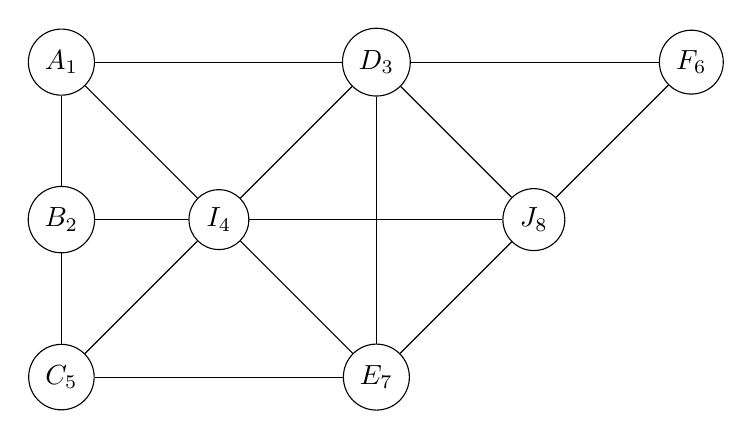
\begin{tikzpicture}
    \draw 
    (1, 1) node[circle, black, draw](C){$C_5$}
    (1, 3) node[circle, black, draw](B){$B_2$}
    (1, 5) node[circle, black, draw](A){$A_1$}
    (3, 3) node[circle, black, draw](I){$I_4$}
    (5, 1) node[circle, black, draw](E){$E_7$}
    (5, 5) node[circle, black, draw](D){$D_3$}
    (7, 3) node[circle, black, draw](J){$J_8$}
    (9, 5) node[circle, black, draw](F){$F_6$};

    \draw[-] (A) -- (B);
    \draw[-] (A) -- (I);
    \draw[-] (A) -- (D);
    \draw[-] (B) -- (I);
    \draw[-] (B) -- (C);
    \draw[-] (C) -- (I);
    \draw[-] (C) -- (E);
    \draw[-] (I) -- (D);
    \draw[-] (I) -- (E);
    \draw[-] (I) -- (J);
    \draw[-] (D) -- (E);
    \draw[-] (D) -- (J);
    \draw[-] (D) -- (F);
    \draw[-] (E) -- (J);
    \draw[-] (J) -- (F);

  \end{tikzpicture}
\end{document}
